\documentclass{article}
\usepackage{fontspec}

% Used to embed Sage code in latex
%\usepackage{sagetex}


% Math Environment
\usepackage{euler}        % Euler font
\usepackage{amsmath}      % Math macros
\usepackage{amssymb}      % Math symbols
\usepackage{unicode-math} % Unicode support

% Physics Environment
\usepackage{physics}


\usepackage[makeroom]{cancel} % Used to cancel terms in algebraic equations
\usepackage{ulem} % Different underline environments
\usepackage{polynom} %Polynomial long division

% Typesetting Rules
\setlength\parindent{0em}
\setlength\parskip{0.618em}
\usepackage[a4paper,lmargin=1in,rmargin=1in,tmargin=1in,bmargin=1in]{geometry}
\setmainfont[Mapping=tex-text]{Helvetica Neue LT Std 45 Light}

% Common Macros
\newcommand\N{\mathbb{N}}
\newcommand\Z{\mathbb{Z}}
\newcommand\Q{\mathbb{Q}}
\newcommand\R{\mathbb{R}}
\newcommand\C{\mathbb{C}}
\newcommand\A{\mathbb{A}}
\def\res{\mathop{\text{Res}}\limits}

% Color
\usepackage[dvipsnames]{xcolor}
\usepackage{pagecolor}
% \definecolor{DeepMossGreen}{HTML}{394820}
% \pagecolor{DeepMossGreen}
% \color{Goldenrod}

\usepackage{graphicx}

\begin{document}

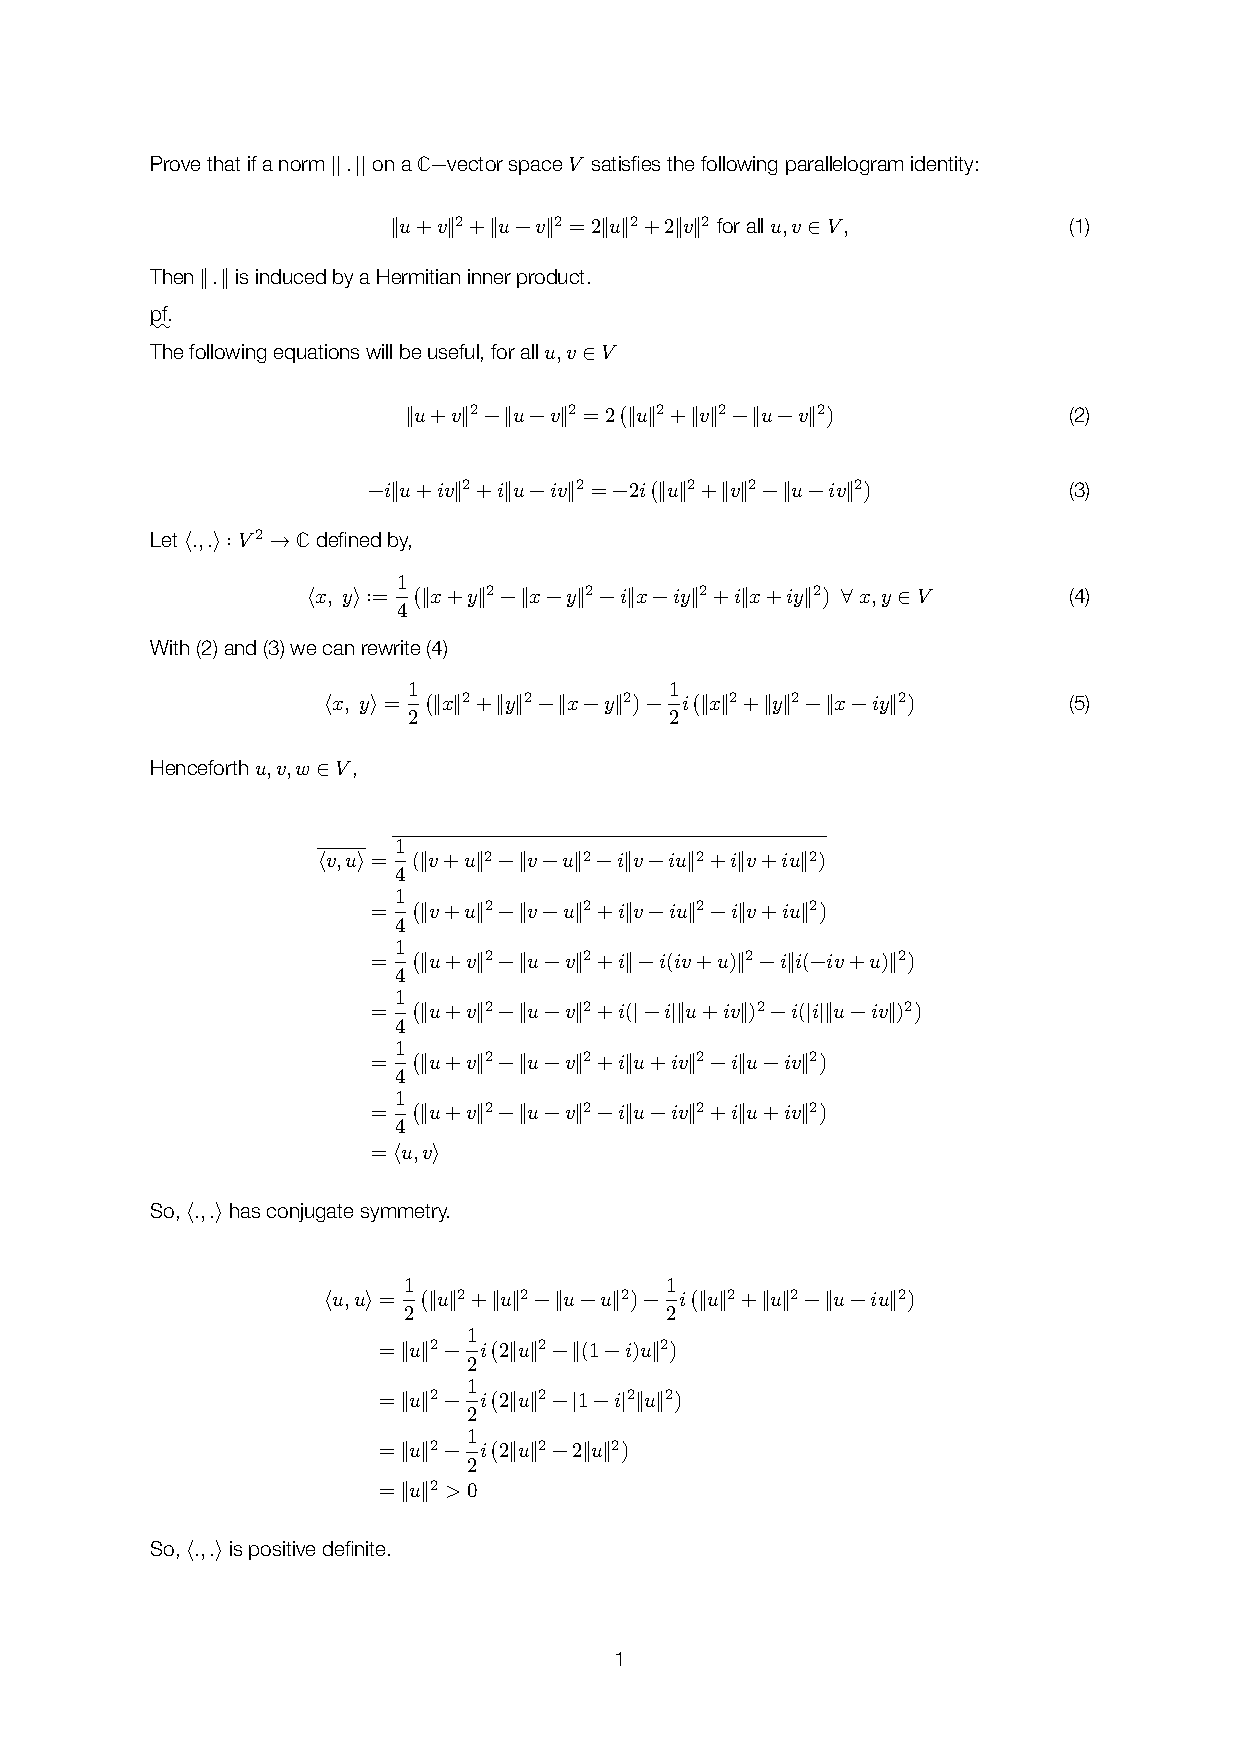
\includegraphics[width=\textwidth]{q1.png}

\uwave{pf.}

We're given $f:E\subset \R^n\rightarrow\R$, such that,
\[\forall \vb{x}\in E,\,\exists M_i\in \R:  |(D_i
f)(\vb{x})| \leq M_i\quad  (1\leq i\leq n).\]

Let $M = \max \{M_1,\dots, M_n\}$, then
\[\forall \vb{x}\in E,\,  |(D_i
f)(\vb{x})| \leq M \quad  (1\leq i\leq n).\]

By (25) if $\{\vb{e}_i\}_{i=1}^n$ is the
standard basis of $\R^n$, we have that
\[\forall \vb{x}\in E,\,  \bigg|\lim_{t\rightarrow 0}
  \frac{f(\vb{x}+t\vb{e}_i) - f(\vb{x})}{t}\bigg| \leq M \quad  (1\leq
  i\leq n).\]

Since $D_i f$ exists for $1\leq i \leq n$,
\begin{align*}
  \bigg|\lim_{t\rightarrow 0}
  \frac{f(\vb{x}+t\vb{e}_i) - f(\vb{x})}{t}\bigg| \leq M
  &\implies  \lim_{t\rightarrow 0}
    \frac{|f(\vb{x}+t\vb{e}_i) - f(\vb{x})|}{|t|} \leq M\\
  &\implies \forall \varepsilon > 0 : |t|<\frac{\varepsilon}{M} \implies  {|f(\vb{x}+t\vb{e}_i) -
    f(\vb{x})|} \leq M |t| \leq  \varepsilon\\
\end{align*}
$|t| = |\vb{x}+t\vb{e}_i -\vb{x}|\implies $  $D_i f$ are continuous on $E$ for $1\leq i\leq n$.

Therefore, by 9.21 $f\in \mathcal{C}'(E)$, since $E\subset \R^n$ is open, and $D_i f$ exists
and are continuous on $E$ for $1\leq i \leq n$.

Then, since $f$ is differentiable on $E$, we can write its derivative
on $E$
as,
\[[f'(\vb{x})] =[ (D_1 f)(\vb{x}) ,\dots, (D_n f)(\vb{x})]\]

Then the operator norm (6), gives,
$$\forall \vb{x}\in E, \exists K \in \R: \|[f'(\vb{x})]\|
  = \{\sum_{i=1}^n (D_i f)(\vb{x})^2\}^{1/2} \leq \{\sum_{i=1}^n
  (M_i)^2\}^{1/2} < K$$

Since $\R^m$ has a countable base by balls, $E =
\cup_{i=1}^\infty B_{r_i}(\vb{x}_i),$ where $  \{x_i\}_{i=1}^\infty$
is sequence in $E$.

Each of the balls are convex open sets, so $f$ satisfies the hypotheses of 9.19 since,
\[\forall x \in B_{r_i}(\vb{x}_i)\quad  \|[f'(\vb{x})]\| < K \]
It follows,
\[|f(\vb{b}) - f(\vb{a})| < M |\vb{b}-\vb{a}|\]
forall $\vb{a},\vb{b} \in B_{r_i}(\vb{x}_i) \subset E$.

Let $\vb{x},\vb{y}\in E$, and let $\varepsilon >0$, then

\[|\vb{y} -\vb{x}|<\frac{\varepsilon}{M}<r_j \implies \exists
  j \in \N:  \vb{x},\vb{y} \in  B_{r_j}(\vb{x}_j) \implies |f(\vb{y}) -
  f(\vb{x})| < M\frac{\varepsilon}{M} = \varepsilon\]

So, $f$ is continuous on $E\quad \blacksquare$

\end{document}



%%% Local Variables:
%%% mode: latex
%%% TeX-master: t
%%% End:
